%In this section we show the important life cycle state machines.
\subsubsection*{Express Lane Check in}
The life cycle state machine for the \texttt{TollLaneExpressCheckIn} class is seen in \autoref{fig:life_cycle_statemachine_toll_lane_computer_express_check_in}. It receives a message from the antenna to indicate that a vehicle with a toll tag has entered the lane. It reacts by sending a message to the station server to check that the tag is valid. If it receives true it tells the station server to check in the tag, opens the barrier, then closes it when the antenna informs it that the tag can no longer be detected.  Otherwise it goes to a faulty tag state and waits for a cashier to resolve the situation. 
\begin{figure}[H]
\centering
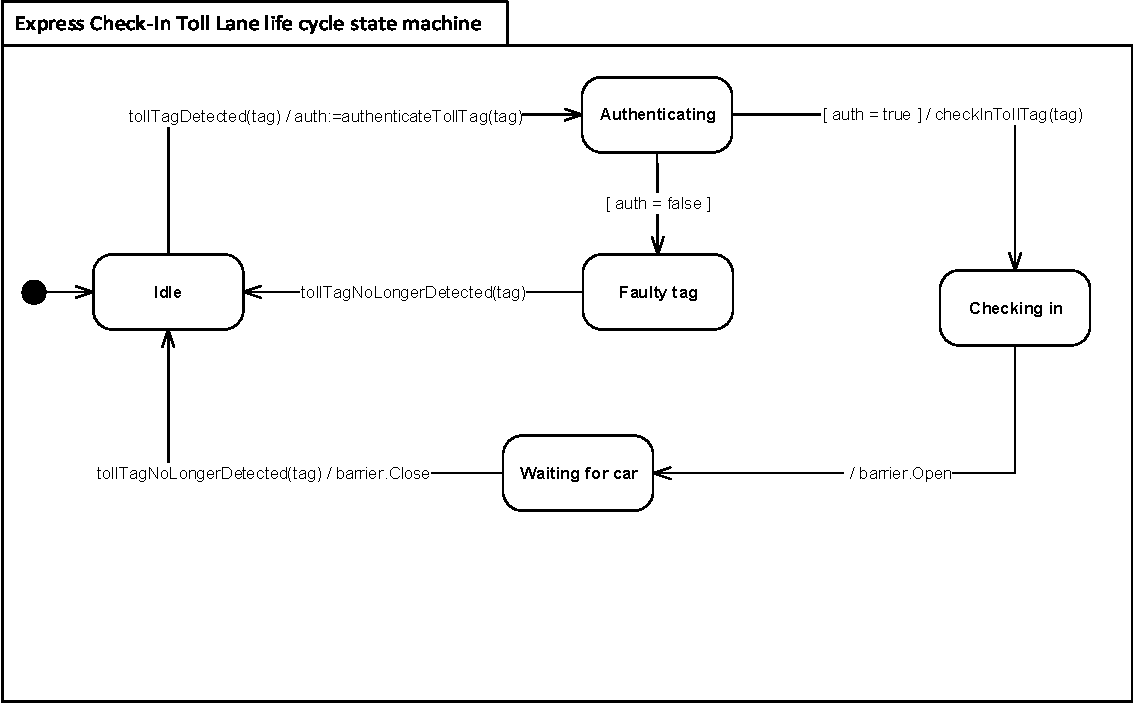
\includegraphics[width=0.7\linewidth]{img/behaviour_state_machines/life_cycle_state_machines/life_cycle_statemachine_toll_lane_computer_express_check_in}
\caption{The life cycle state machine for the \texttt{TollLaneExpressCheckIn} class}
\label{fig:life_cycle_statemachine_toll_lane_computer_express_check_in}
\end{figure}

\subsubsection*{Express Lane Check out}
The life cycle state machine for the \texttt{TollLaneExpressCheckOut} class is seen in \autoref{fig:life_cycle_statemachine_toll_lane_computer_express_check_in}. It receives a message from the antenna to indicate that a vehicle with a toll tag has entered the lane. It reacts by sending a message to the station server to check that the tag is checked in. If it receives true it tells the station server to check out the tag, opens the barrier, then closes it when the antenna informs it that the tag can no longer be detected.  Otherwise it goes to a faulty tag state and waits for a cashier to resolve the situation. 
\begin{figure}[H]
\centering
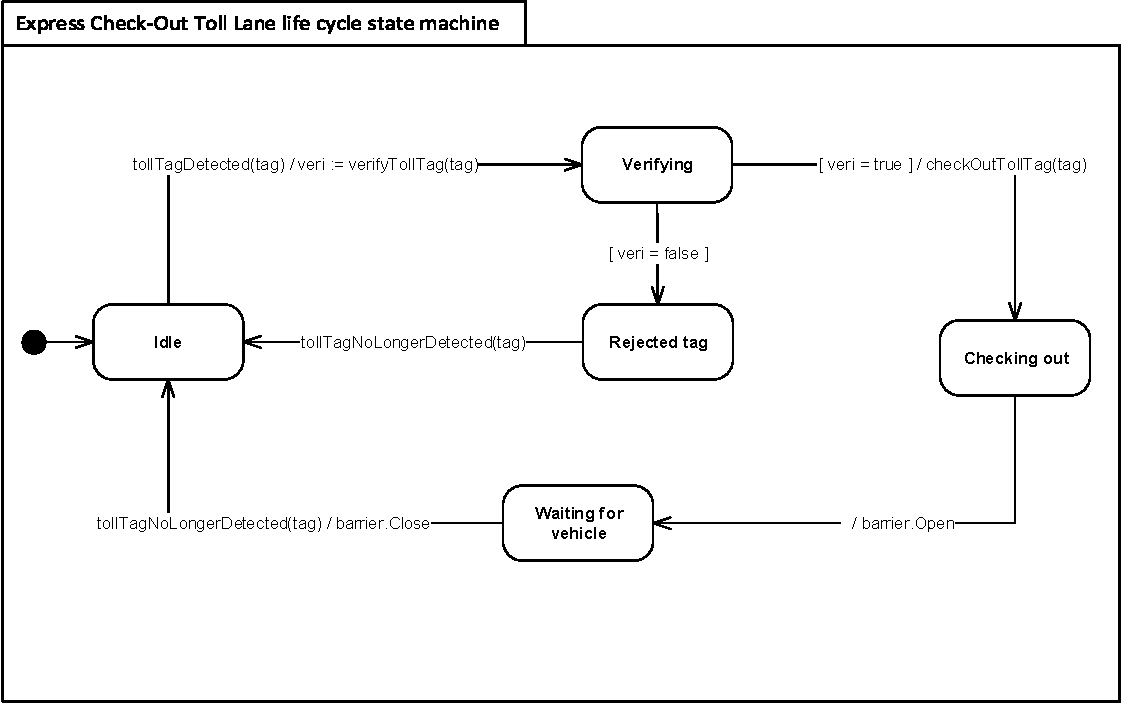
\includegraphics[width=0.7\linewidth]{img/behaviour_state_machines/life_cycle_state_machines/life_cycle_statemachine_toll_lane_computer_express_check_out}
\caption{The life cycle state machine for the \texttt{TollLaneExpressCheckOut} class}
\label{fig:life_cycle_statemachine_toll_lane_computer_express_check_out}
\end{figure}

\subsubsection*{Normal Lane Check in}
The life cycle state machine for the \texttt{TollLaneNormalCheckIn} class is seen in \autoref{fig:life_cycle_statemachine_toll_lane_computer_express_check_in}. It waits for the touch screen to send information about a vehicle. It returns the price for that vehicle, then waits to receive payment via cash or credit card. If payment is received via card, it contacts the bank about the transaction. It then prints a ticket and opens the barrier long enough for the customer to pass.
\begin{figure}[H]
\centering
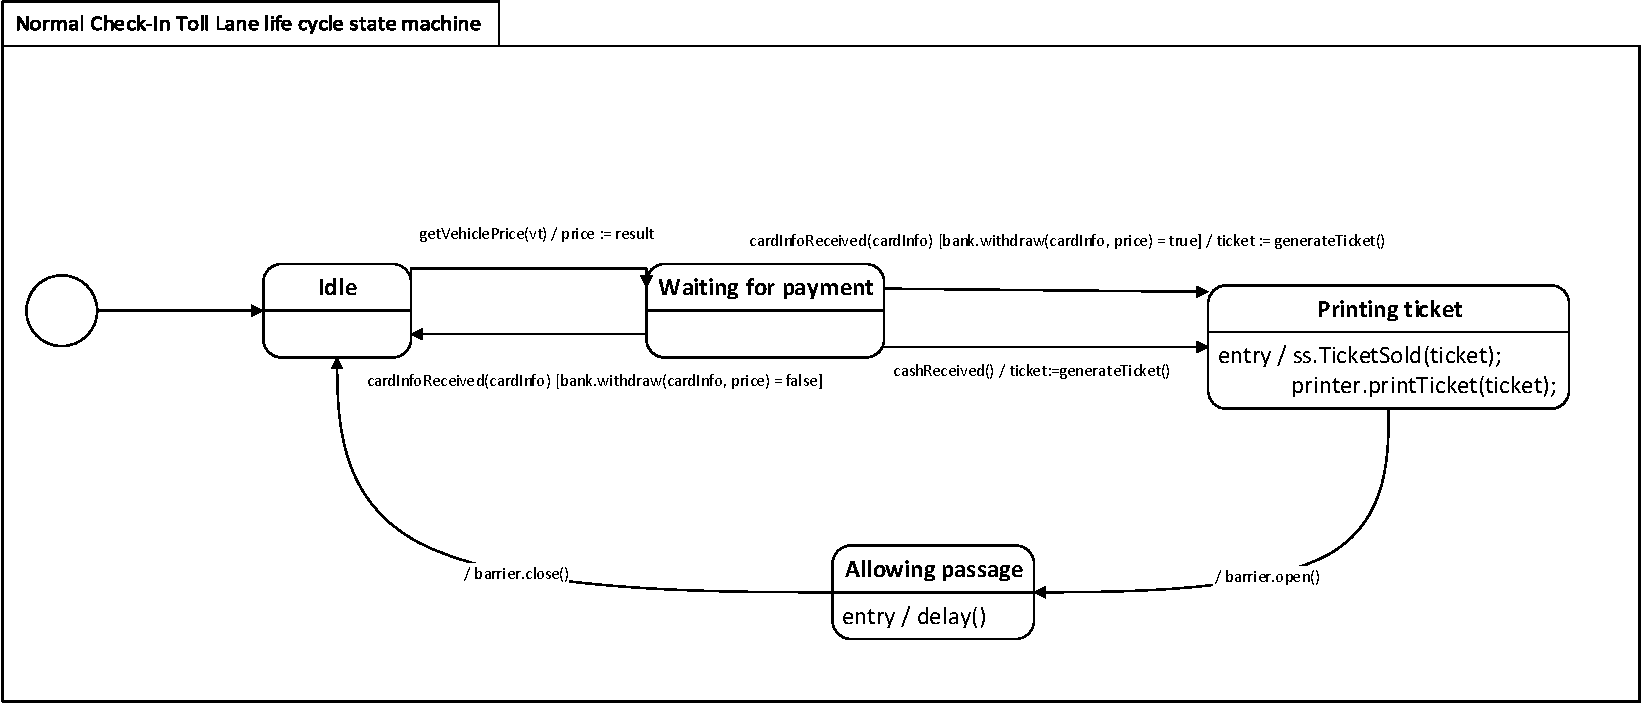
\includegraphics[width=0.7\linewidth]{img/behaviour_state_machines/life_cycle_state_machines/life_cycle_state_machine_toll_lane_computer}
\caption{The life cycle state machine for the \texttt{TollLaneNormalCheckIn} class}
\label{fig:life_cycle_state_machine_toll_lane_computer}
\end{figure}

\subsubsection*{Normal Lane Check out}
The life cycle state machine for the \texttt{TollLaneNormalCheckOut} class is seen in \autoref{fig:life_cycle_statemachine_toll_lane_computer_express_check_in}. It waits for a ticket to be inserted. When it is, it contacts the station server to validate the ticket. If the ticket is valid, it opens the barrier, waits for the customer to leave, then closes the barrier. Otherwise it goes to an invalid ticket state and waits for a cashier to resolve the situation.
\begin{figure}[H]
\centering
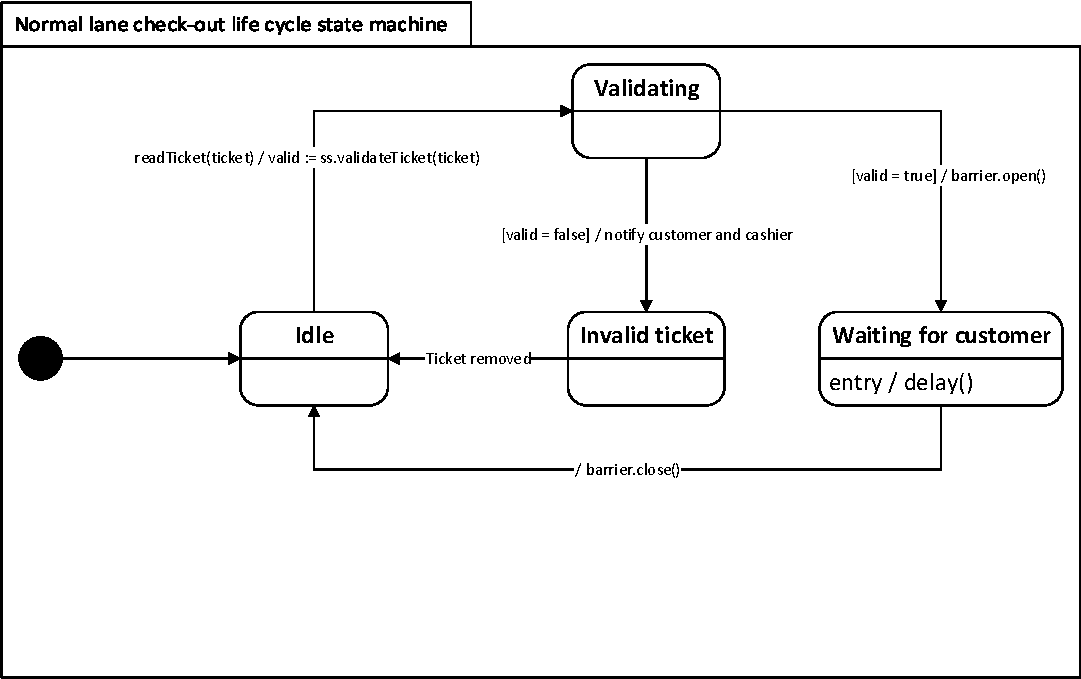
\includegraphics[width=0.7\linewidth]{img/behaviour_state_machines/life_cycle_state_machines/life_cycle_state_machine_toll_computer_normal_lane}
\caption{The life cycle state machine for the \texttt{TollLaneNormalCheckOut} class}
\label{fig:life_cycle_state_machine_toll_computer_normal_lane}
\end{figure}

\subsubsection*{Station server}
The life cycle state machine for the \texttt{StationServer} class is seen in \autoref{fig:life_cycle_statemachine_toll_lane_computer_express_check_in}. It sends messages between the Toll Lane and the Enterprise Server.
\begin{figure}[H]
\centering
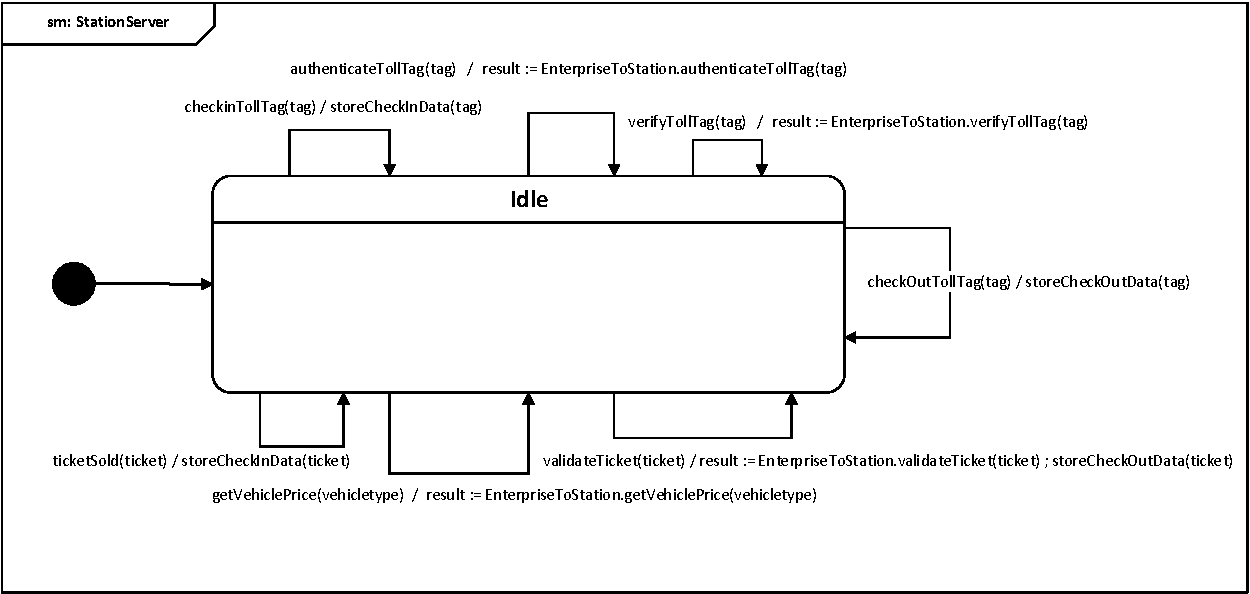
\includegraphics[width=0.7\linewidth]{img/behaviour_state_machines/life_cycle_state_machines/life_cycle_state_machine_station_server}
\caption{The life cycle state machine for the \texttt{StationServer} class}
\label{fig:life_cycle_state_machine_station_server}
\end{figure}


\subsubsection*{Enterprise server}
As the functionality of the enterprise server is quite complex we have split up its functionality into multiple diagrams. Each diagram shows the same concurrent state \texttt{Working}, meaning that all parts of all the diagrams are running concurrently. In the following we will go into detail for each diagram.

\paragraph*{Part 1} In \autoref{fig:life_cycle_state_machine_enterprise_server} we first show the part which handles customers buying toll tags online through the web server. The customer fills out the form and if his credit card information can be validated the data is stored and the order for the toll tag is placed.

Next we show how reports are compiled for the enterprise manager.

Finally we show how the enterprise server authenticates toll tags. First the server authenticates that the toll tag is issued and then it checks  whether the toll tag is expired.

\begin{figure}[H]
\centering
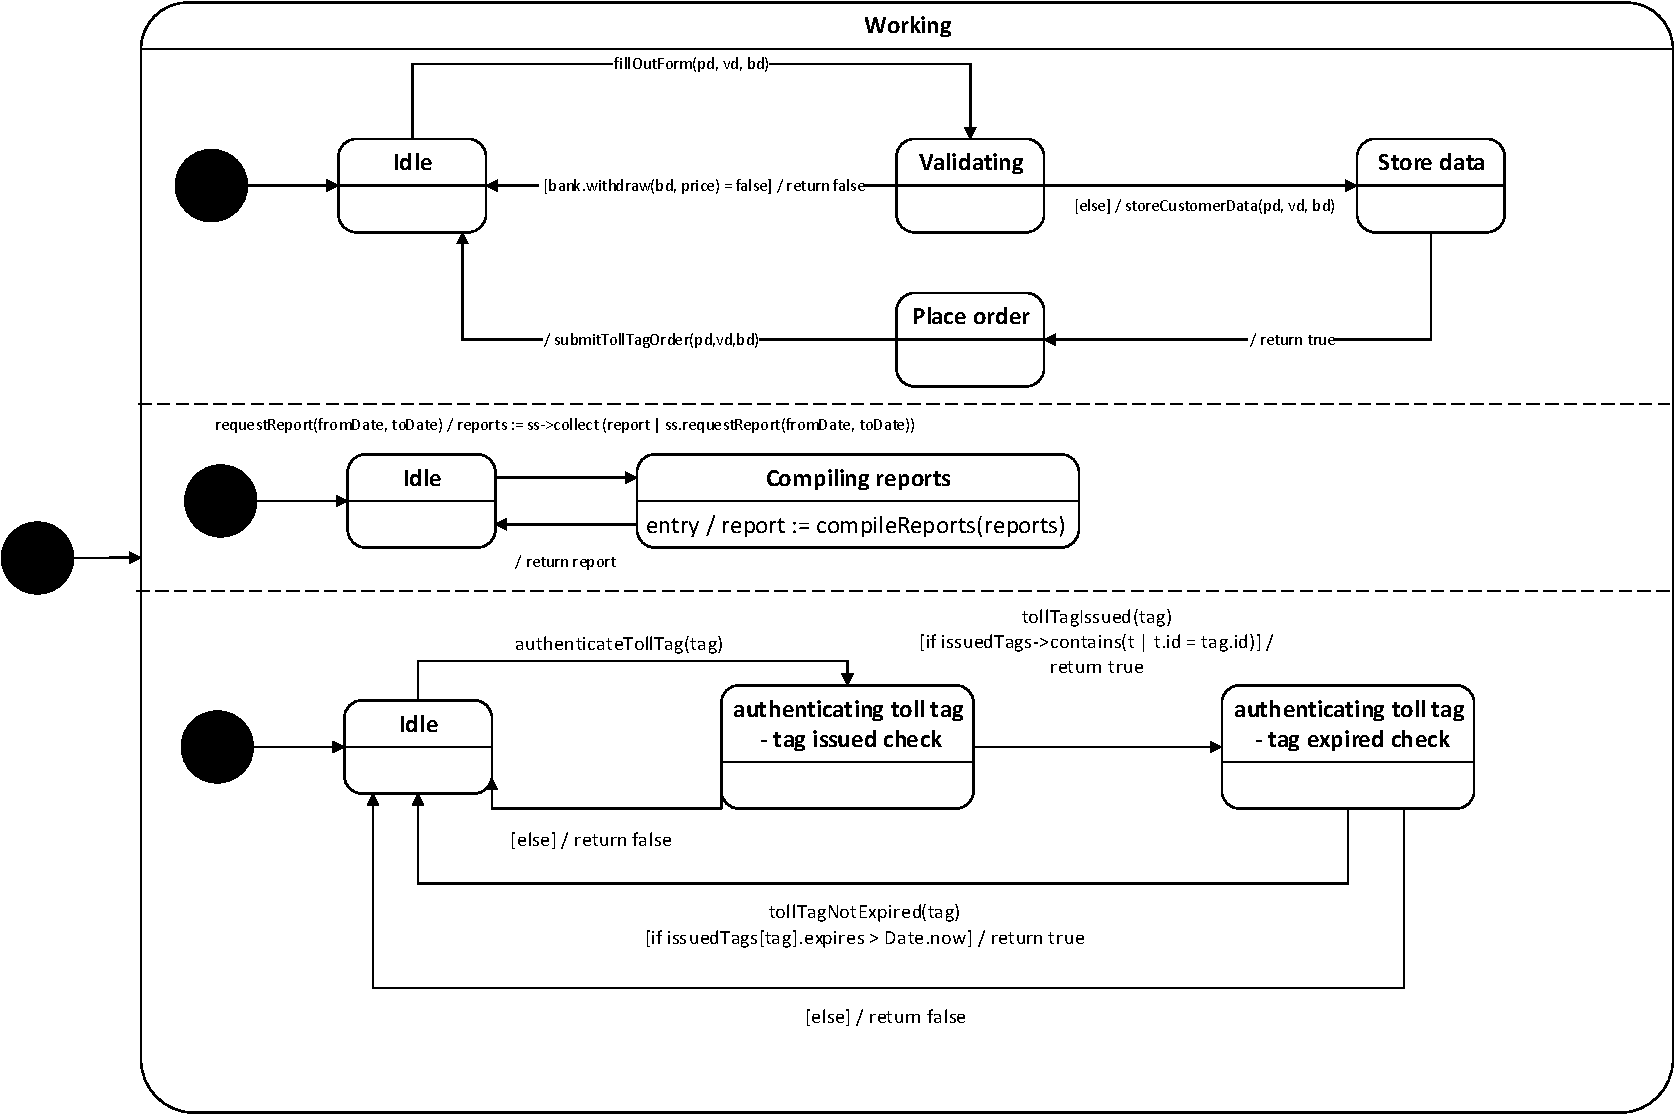
\includegraphics[width=0.7\linewidth]{img/behaviour_state_machines/life_cycle_state_machines/life_cycle_state_machine_enterprise_server}
\caption{The life cycle state machine for the \texttt{EnterpriseServer} class}
\label{fig:life_cycle_state_machine_enterprise_server}
\end{figure}

\paragraph*{Part 2} In \autoref{fig:life_cycle_state_machine_enterprise_server_part2} we show how the enterprise server handles check in with a toll tag. For check in we register the relevant information for doing a check out. We also show how the enterprise verifies that a toll tag has been checked in. This is to be used before the toll tag can be properly checked out.

\begin{figure}[H]
\centering
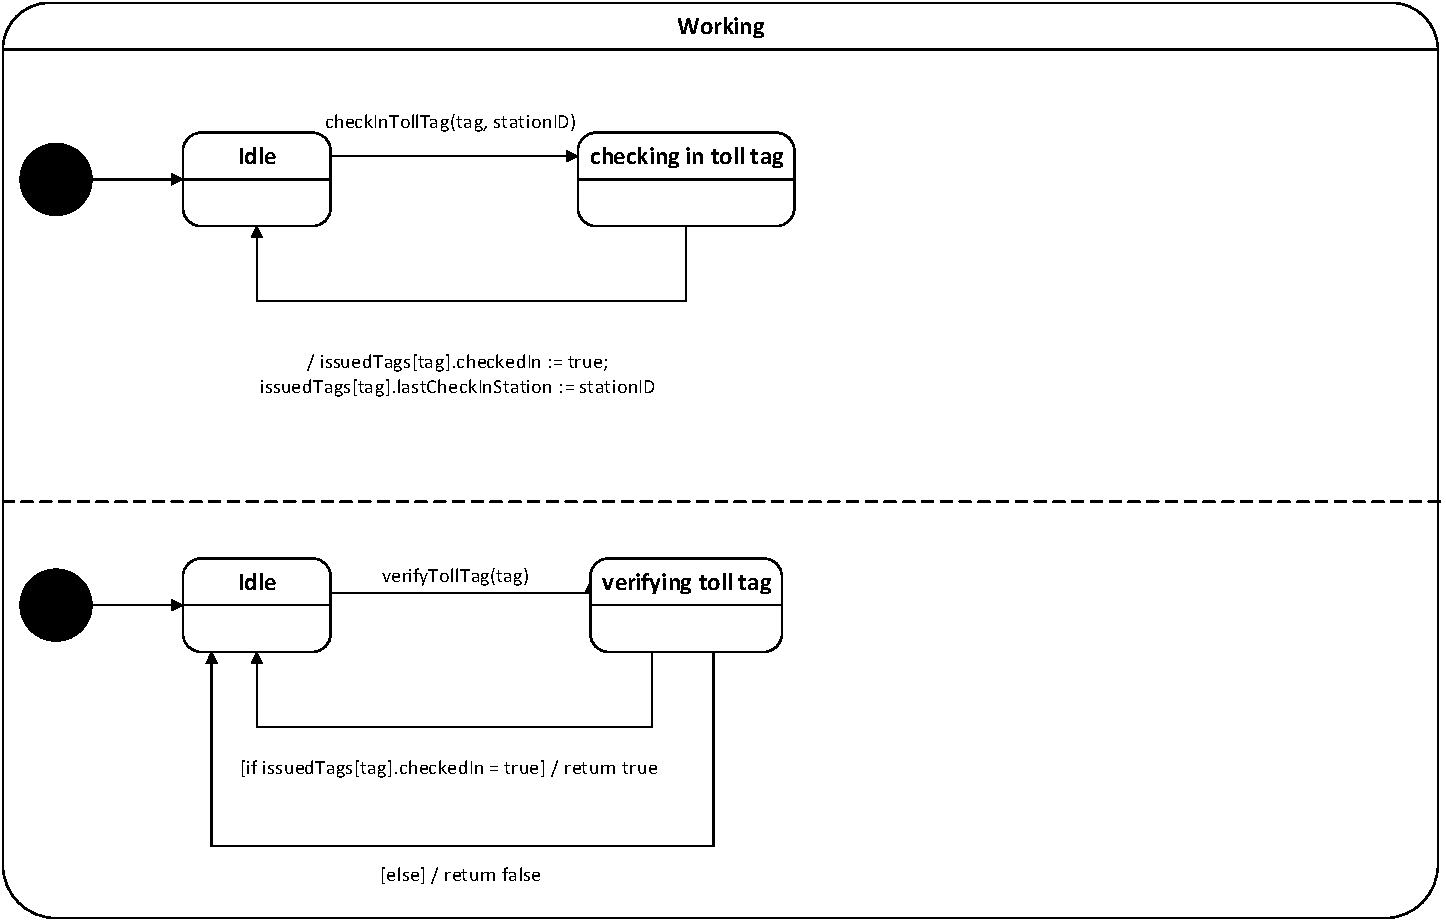
\includegraphics[width=0.7\linewidth]{img/behaviour_state_machines/life_cycle_state_machines/life_cycle_state_machine_enterprise_server_part2}
\caption{The life cycle state machine for the \texttt{EnterpriseServer} class}
\label{fig:life_cycle_state_machine_enterprise_server_part2}
\end{figure}

\paragraph*{Part 3} In \autoref{fig:life_cycle_state_machine_enterprise_server_part3} we first show how to check out with single tickets. The enterprise server validates the ticket and then removes it from the database on the enterprise server making the validation check fail if the customer attempts to use it again.
\\
We then show how to check out a toll tag. The check out is performed after the toll tag has been verified.
\\
Finally we show what happens when a ticket is sold.

\begin{figure}[H]
\centering
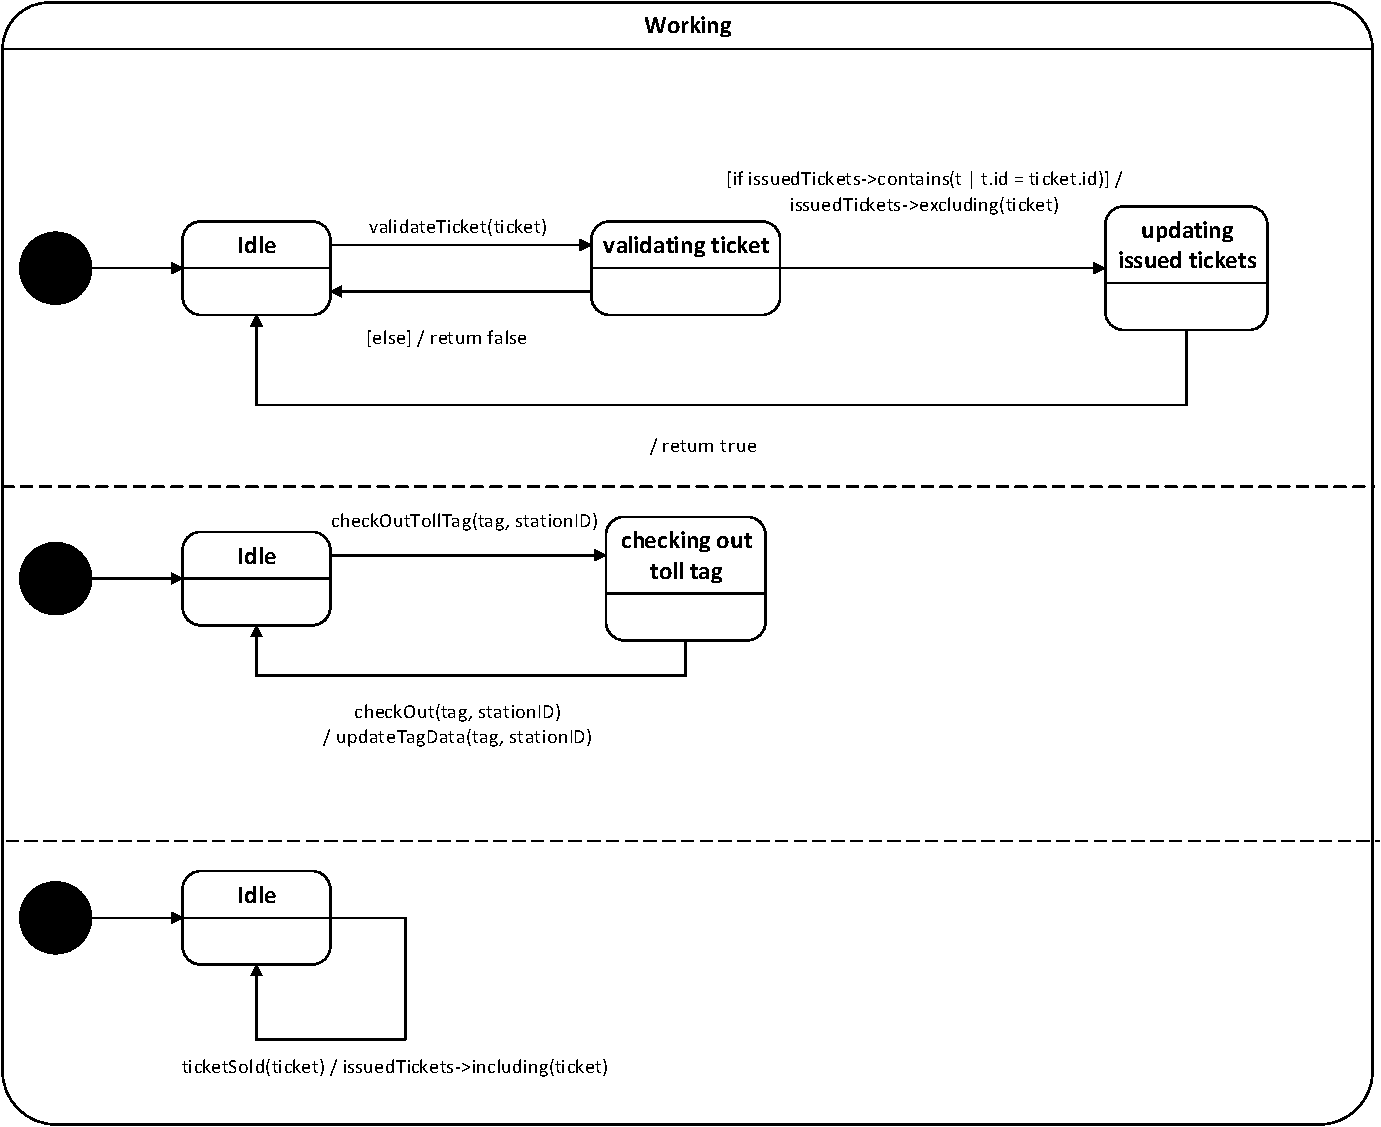
\includegraphics[width=0.7\linewidth]{img/behaviour_state_machines/life_cycle_state_machines/life_cycle_state_machine_enterprise_server_part3}
\caption{The life cycle state machine for the \texttt{EnterpriseServer} class}
\label{fig:life_cycle_state_machine_enterprise_server_part3}
\end{figure}